\documentclass{beamer}
\usepackage{tikz}
\usetikzlibrary{arrows,shapes,matrix,positioning}

\begin{document}

\begin{frame}[fragile]{La matrice tableau di un PL in forma canonica}
\centering
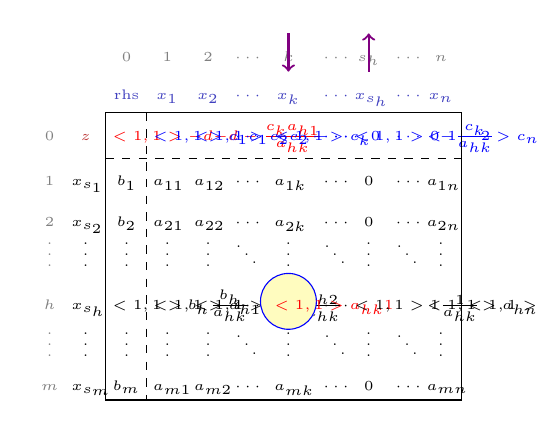
\begin{tikzpicture}
{\tiny
\node[%
  align=center,
  row 1/.style=gray,
  row 2/.style=blue!50!gray,
  row 3/.style={blue},
  column 1/.style={gray,text width=1em},
  column 2/.style={red!50!gray,text width=1em}
  column 3/.style={red,text width=6em},
  column 6/.style={text width=1em},
  column 8/.style={text width=1em},
  column 10/.style={text width=1em},
  row 3 column 1/.style={gray},
  row 3 column 2/.style={red!50!gray},
  row 3 column 3/.style={red},
  text width=1.5em,
  text height=3.5ex,
  matrix of math nodes] (M)
{%
% Indice delle righe (M-1)
~&~&0&1&2&\cdots&k&\cdots&s_h&\cdots&n\\
% Intestazione delle colonne (M-2)
~ &~&  \mbox{rhs}&  x_1 &  x_2 &  \cdots &  x_k &  \cdots &  x_{s_h} &  \cdots &  x_n & ~\\
% Riga 0, fo e costi ridotti (M-3)
0 & z & \alt<1,1>{-d}{-d-\frac{c_k a_{h1}}{a_{hk}}} & \alt<1,1>{c_1}{c_1-\cdots} & \alt<1,1>{c_2}{c_2-\cdots} & \cdots & \alt<1,1>{c_k}{0} & \cdots & \alt<1,1>{0}{-\frac{c_k}{a_{hk}}} & \cdots &  \alt<1-2>{c_n}{c_n-\frac{c_k a_{hn}}{a_{hk}}} & \\
1& x_{s_1} & b_1 &  a_{11} &  a_{12} &  \cdots &  a_{1k} &  \cdots &  0&  \cdots &  a_{1n} & ~\\
2& x_{s_2} & b_2 &  a_{21} &  a_{22} &  \cdots &  a_{2k} &  \cdots &  0 &  \cdots & a_{2n} & ~\\
\vdots & \vdots &  \vdots &  \vdots &  \vdots &  \ddots &  \vdots &  \ddots &  \vdots &\ddots  & \vdots & ~\\
h& x_{s_h} & \alt<1,1>{b_h}{\frac{b_h}{a_{hk}}} &  \alt<1,1>{a_{h1}}{\frac{a_{h1}}{a_{hk}}} &  \alt<1,1>{a_{h2}}{\frac{a_{h2}}{a_{hk}}} &  \cdots &  \node[red, draw=blue, shape=circle,fill=yellow!25,opacity=1] {\alt<1,1>{a_{hk}}{1}}; &  \cdots &  \alt<1,1>{1}{\frac{1}{a_{hk}}} &  ~ & \alt<1,1>{a_{hn}}{\frac{a_{hn}}{a_{hk}}} & \alt<1,1>{}{{\mathbf{A}_h} \gets \frac{1}{a_{hk}} {\mathbf{A}_h}} \\
\vdots& \vdots &  \vdots &  \vdots &  \vdots &  \ddots &  \vdots &  \ddots &\vdots & \ddots&\vdots & ~\\
m& x_{s_m} & b_m &  a_{m1} &  a_{m2} &  \cdots &  a_{mk} &  \cdots &  0 &  \cdots& a_{mn} & ~\\
};

\uncover<2->{
% entra x_k
\draw[->,thick,red!50!blue] (M-1-7.north) to (M-2-7.north);
% esce x_{s_h}
\draw[->,thick,red!50!blue] (M-2-9.north) to (M-1-9.north);
}

% riquadro
\draw(M-3-3.north west) -- (M-3-11.north east) -- (M-9-11.south east) -- (M-9-3.south west) -- cycle;

% separatore orizzontale
\draw[dashed] (M-4-3.north west) -- (M-4-11.north east);

% separatore verticale
\draw[dashed] (M-3-4.north west) -- (M-9-4.south west);

%% A_s: 3--8: 9--14
%\uncover<2->{
%\fill[red!50,fill opacity=0.5,thick,draw=red!60!black]  (M-3-9.north west) rectangle (M-8-14.south east);
%\node[red!40!black, below = of M-8-11.north east,draw=red!40,thick] (as) {$\alpha)\ \mathbf{A}_S = \mathbf{I}_m$};
%\draw[->,red!60,thick] (as) to (M-5-11.east);
%}
%% c_s: 2: 9--12
%\onslide<3->{
%\fill[green!50,fill opacity=0.5,thick,draw=green!60!black]  (M-2-9.north west) rectangle (M-2-14.south east);
%\node[green!40!black, above = of M-2-11.south east,draw=green!40,thick] (cs) {$\beta)\ \mathbf{c}_S = \mathbf{0}$};
%\draw[->,green!60,thick] (cs) to (M-2-11.east);
%}
%% b: 3--8: 2
%\uncover<4->{
%\fill[blue!50,fill opacity=0.5,thick,draw=blue!60!black]  (M-3-2.north west) rectangle (M-8-2.south east);
%\node[blue!40!black, below = of M-8-2.north,draw=blue!40,thick] (b) {$\gamma\ \mathbf{b} \geq \mathbf{0}$};
%\draw[->,blue!60,thick] (b) to [out=180,in=180] (M-5-2);
%}
}
\end{tikzpicture}
%sono fragile: lasciami uno spazio vuoto

\end{frame}
\end{document}
